\documentclass[mat1, tisk]{fmfdelo}
\usepackage{amsmath}
\usepackage{graphicx}
\usepackage{hyperref}
% \documentclass[fin1, tisk]{fmfdelo}
% Če pobrišete možnost tisk, bodo povezave obarvane,
% na začetku pa ne bo praznih strani po naslovu, …

%%%%%%%%%%%%%%%%%%%%%%%%%%%%%%%%%%%%%%%%%%%%%%%%%%%%%%%%%%%%%%%%%%%%%%%%%%%%%%%
% METAPODATKI
%%%%%%%%%%%%%%%%%%%%%%%%%%%%%%%%%%%%%%%%%%%%%%%%%%%%%%%%%%%%%%%%%%%%%%%%%%%%%%%

% - vaše ime
\avtor{Manca Murn}

% - naslov dela v slovenščini
\naslov{Metrična dimenzija leksikografskega produkta grafov}

% - naslov dela v angleščini
\title{The metric dimension of the lexicographic product of graphs}

% - ime mentorja/mentorice s polnim nazivom:
%   - doc.~dr.~Ime Priimek
%   - izr.~prof.~dr.~Ime Priimek
%   - prof.~dr.~Ime Priimek
%   za druge variante uporabite ustrezne ukaze
\mentor{Sandi Klavžar}
% \somentor{...}
% \mentorica{...}
% \somentorica{...}
% \mentorja{...}{...}
% \somentorja{...}{...}
% \mentorici{...}{...}
% \somentorici{...}{...}

% - leto diplome
\letnica{2023} 

% - povzetek v slovenščini
%   V povzetku na kratko opišite vsebinske rezultate dela. Sem ne sodi razlaga
%   organizacije dela, torej v katerem razdelku je kaj, pač pa le opis vsebine.
\povzetek{...}

% - povzetek v angleščini
\abstract{... }

% - klasifikacijske oznake, ločene z vejicami
%   Oznake, ki opisujejo področje dela, so dostopne na strani https://www.ams.org/msc/
\klasifikacija{..., ...}

% - ključne besede, ki nastopajo v delu, ločene s \sep
\kljucnebesede{...\sep ...}

% - angleški prevod ključnih besed
\keywords{...\sep ...} % angleški prevod ključnih besed

% - angleško-slovenski slovar strokovnih izrazov
\slovar{
% \geslo{angleški izraz}{slovenski izraz}
% ...
}

% - ime datoteke z viri (vključno s končnico .bib), če uporabljate BibTeX
% \literatura{....bib}

%%%%%%%%%%%%%%%%%%%%%%%%%%%%%%%%%%%%%%%%%%%%%%%%%%%%%%%%%%%%%%%%%%%%%%%%%%%%%%%
% DODATNE DEFINICIJE
%%%%%%%%%%%%%%%%%%%%%%%%%%%%%%%%%%%%%%%%%%%%%%%%%%%%%%%%%%%%%%%%%%%%%%%%%%%%%%%

% naložite dodatne pakete, ki jih potrebujete
% \usepackage{...}

% deklarirajte vse matematične operatorje, da jih bo LaTeX pravilno stavil
% \DeclareMathOperator{\...}{...}

% vstavite svoje definicije ...
% \newcommand{\...}{...}


%%%%%%%%%%%%%%%%%%%%%%%%%%%%%%%%%%%%%%%%%%%%%%%%%%%%%%%%%%%%%%%%%%%%%%%%%%%%%%%
% ZAČETEK VSEBINE
%%%%%%%%%%%%%%%%%%%%%%%%%%%%%%%%%%%%%%%%%%%%%%%%%%%%%%%%%%%%%%%%%%%%%%%%%%%%%%%

\begin{document}

\section{Uvod}
V decembru leta 2010 sta v razmaku 17 dni nastala dva različna članka z enakim naslovom - 
\textit{"The metric dimension of the lexicographic product of graphs"}. Avtorji obeh člankov 
bojda niso vedeli za delo drugega in so se teme lotili na dva posvem različna načina. 
V tem diplomskem seminarju si bomo ogledali pojem metrične dimenzije grafa in njene osnovne 
lastnosti, definirali leksikografski produkt grafov ter povzeli glavne rezultate o metrični 
dimenziji leksikografskega produkta iz obeh člankov. Na koncu bomo skušali najti tudi 
povezavo med enim in drugim pristopom obravnave le te. 


%%%%%%%%%%%%%%%%%%%%%%%%%%%%%%%%%%%%%%%%%%%%%%%%%%%%%%%%%%%%%%%%%%%%%%%%%%%%%%%
%%%%%%%%%%%%%%%%%%%%%%%%%%%%%%%%%%%%%%%%%%%%%%%%%%%%%%%%%%%%%%%%%%%%%%%%%%%%%%%


\subsection{Osnovni pojmi} \label{ss:osnovni_pojmi}
Za začetek ponovimo nekaj osnovnih definicij in oznak iz teorije grafov, ki jih bomo potrebovali 
za razumevanje tega diplomskega seminarja. 

\begin{definicija} \label{def:graf}
    Graf $G$ je urejen par $(V(G), E(G)),$ kjer je $V(G)$ množica vozlišč in $E(G)$ 
    podmnožica v $\binom{V(G)}{2},$ ki vsebuje povezave grafa.
\end{definicija}

Če je $V(G)$ končna množica, je $G$ končen graf. Število $|V(G)|$ imenujemo red grafa. 
Če je med dvema različnima vozliščema največ ena povezava in nobeno vozlišče ni povezano samo 
s seboj, pravimo, da je graf enostaven. Vozlišči $v, u \in G$ sta sosedni, če $uv \in E(G).$ 
Sosednost je ekvivalenčna relacija, zato sosedni vozlišči označimo $u \sim v.$ Če $w, x \in V(G)$ 
nista sosedni pa pišemo $w \not \sim x.$

\begin{definicija} \label{def:komplement}
    Komplement grafa $G$, je graf $\overline{G},$ za katerega velja $V(G) = V(\overline{G})$ in 
    $$\forall u,v \in V(\overline{G}): uv E(\overline{G}) \Leftrightarrow uv \not \in E(G).$$
\end{definicija}

Sprehod v grafu $G$ je zaporedje vozlišč $v_1, v_2, ... v_k$ iz $V(G)$, tako da je 
$\forall i : v_i, v_{i+1} \in E(G).$ Sprehod je enostaven, če vsebuje sama različna vozlišča.
Graf je povezan, če med vsakima dvema različnima vozliščema obstaja sprehod. Na povezanem
grafu lahko definiramo razdaljo med vozliščema.

\begin{definicija} \label{def:razdalja}
    Razdalja med dvema vozliščema $u, v \in V(G)$ je dolžina najkrajšega sprehoda in jo 
    označujemo z $d(u, v).$ 
\end{definicija}

Naslednja trditev o razdaji med vozlišči je očitna.

\begin{trditev} \label{trd:nicelna_razdalja}
    Za povezan graf $G$ in poljubni vozlišči $v, w \in V(G)$ velja:
    $$ d(v, w) = 0 \Leftrightarrow v=w.$$
\end{trditev} 

\begin{definicija} \label{def:podgraf}
    Graf $H$ je podgraf grafa $G$ natanko tedaj, ko velja $V(H) \subseteq V(G)$ in 
    $E(H) \subseteq E(H)$.
\end{definicija}

\begin{definicija} \label{def:induciran_podgraf}
    Graf $H$ je induciran podgraf grafa $G$ natanko tedaj, ko velja 
    $\forall u, v \in V(H) : uv \in E(G) \Rightarrow E(H)$.
\end{definicija}

\begin{definicija} \label{def:komponenta}
Komponenta grafa je povezan podgraf, ki ni del nobenega večjega povezanega podgrafa. 
\end{definicija}

Povezan graf ima seveda samo eno komponento. Definirajmo še operacijo združitve grafov.

\begin{definicija} \label{def:vsota}
    Vsota grafov $G$ in $H$, je graf $G + H$, za katerega velja $V(G + H) = V(G) \cup V(H)$ 
    in $E(G + H)  = E(G) \cup E(H) \cup \{ uv \;  | \;  u \in V(G) \land v \in V(H) \}.$
\end{definicija}
%je to ime vredu? v angleščini je joint graphs...

Poglejmo še nekaj primerov osnovnih razredov grafov:
\begin{itemize} \label{primeri_grafov}
    \item Prazen graf na $n$ vozliščih, ki ga označujemo z $N_n$, nima nobenih povezav. 
    \item Polni graf na $n$ vozliščih, ki ga označujemo z $K_n$, ima vse možne povezave.
    \item Polni dvodelni graf, ki ga označujemo z $K_{n, m}$ ima množico 
    vozlišč $V(K_{n,m}) = \{ v_1, v_2, ... , v_n , u_1, u_2, ... , u_m \}$
    in povezave $E(K_{n, m}) = \{ v_i u_j \; | \;  1 \leq i \leq n \; \land \; 1 \leq j \leq m \}.$ 
    \item Zvezda na $n$ vozliščih je poseben primer polnega dvodelnega grafa in jo označujemo
    z $S_{(n-1)} = K_{1, (n-1)}$
    \item Pot na $n$ vozliščih, ki jo označujemo z $P_n$, ima množico povezav 
    $E(P_n) = \{ v_1 v_2 , v_2 v_3 , ... , v_{n-1} v_n\}.$
    \item Cikel na $n$ vozliščih, dobimo tako, da grafu $P_n$ dodamo povezavo $n 1$.
    \item IME?? na $k+l$ vozliščih je enak združitvi poti in praznega grafa in ga označujemo s 
    $F_{k,l} = N_k + P_l.$
    %fan graph
    \item Drevo je povezan graf, ki ne vsebuje nobenega cikla.
\end{itemize}

\begin{opomba}
    Očitno velja $P_1 = K_1 = N_1 = C_1.$ To je graf s samo enim vozliščem. Običajno ga bomo
    označevali s $K_1.$
\end{opomba}


%%%%%%%%%%%%%%%%%%%%%%%%%%%%%%%%%%%%%%%%%%%%%%%%%%%%%%%%%%%%%%%%%%%%%%%%%%%%%%%
%%%%%%%%%%%%%%%%%%%%%%%%%%%%%%%%%%%%%%%%%%%%%%%%%%%%%%%%%%%%%%%%%%%%%%%%%%%%%%%
%%%%%%%%%%%%%%%%%%%%%%%%%%%%%%%%%%%%%%%%%%%%%%%%%%%%%%%%%%%%%%%%%%%%%%%%%%%%%%%
%%%%%%%%%%%%%%%%%%%%%%%%%%%%%%%%%%%%%%%%%%%%%%%%%%%%%%%%%%%%%%%%%%%%%%%%%%%%%%%


\section{Metrična dimenzija grafa} \label{s:metricna_dim_grafa}

%motivacija neki izvirnega
TODO - motivacija

%%%%%%%%%%%%%%%%%%%%%%%%%%%%%%%%%%%%%%%%%%%%%%%%%%%%%%%%%%%%%%%%%%%%%%%%%%%%%%%
%%%%%%%%%%%%%%%%%%%%%%%%%%%%%%%%%%%%%%%%%%%%%%%%%%%%%%%%%%%%%%%%%%%%%%%%%%%%%%%


\subsection{Definicija} \label{ss:definicija_metricne_dim_grafa}

Metrična dimenzija grafa je najmanjše število vozlišč grafa, ki jih potrebujemo, da
vsa vozlišča v grafu razlikujemo med sabo zgolj s pomočjo razdalj do izbranih vozlišč.
V matematičnem jeziku to povemo takole:

\begin{definicija} \label{def:metricna_predstavitev}
    Naj bo $G$ povezan graf in $W = \{ w_1, ... , w_k  \} \subseteq V(G)$ neprazna 
    podmnožica vozlišč. Vektor $r_W(v) = (d(v, w_1), ..., d(v, w_k))$ imenujemo metrična 
    predstavitev vozlišča $v \in V(G)$ s podmnožico $W$.
\end{definicija}

\begin{definicija} \label{def:resljiva_mn}
    Neprazna podmnožica $R \subseteq V(G)$ je rešljiva,
    če $\forall u, v \in V(G): u \neq v \implies r_R(v) \neq r_R(u)$.
\end{definicija}

\begin{definicija} \label{def:baza_dimenzija}
    Najmanjša rešljiva množica grafa $G$ se imenuje metrična baza. Njeno velikost imenujemo 
    metrična dimenzija in jo označimo z $\beta(G).$ 
\end{definicija}

Poglejmo si nekaj lahkih osnovnih primerov.


\begin{primer} \label{pr:mdim_pot}
Označimo vozlišča poti z $v_1, v_2, ..., v_n$, kot je prikazano na spodnji sliki \ref{fig:pot}. 
Izberimo podmnožico $W = \{v_1\} \subseteq V(G).$ Metrične predstavitve vozlišč grafa $P_n$, 
glede na $W$, so potem sledeče:
\begin{align*}
    r_W(v_1) = d(v_1, v_1) & = 0 \\
    r_W(v_2) = d(v_2, v_1) & = 1 \\
    & \dots \\
    r_W(v_{n-1}) = d(v_{n-1}, v_1) & = n-2 \\
    r_W(v_n) = d(v_n, v_1) & = n-1.
\end{align*}

Vidimo, da so metrične predstavitve vseh vozlišč med seboj različne. Sledi, da je $W$ 
rešljiva množica. Ker je njena velikost enaka $1$ in je to najmanjša možna neprazna podmnožica 
vozlišč, je torej metrična dimenzija grafa poti poljubne dolžine enaka $\beta(P_n) = 1.$

\begin{figure}[h]
    \caption{Graf $P_5$}
    \centering
    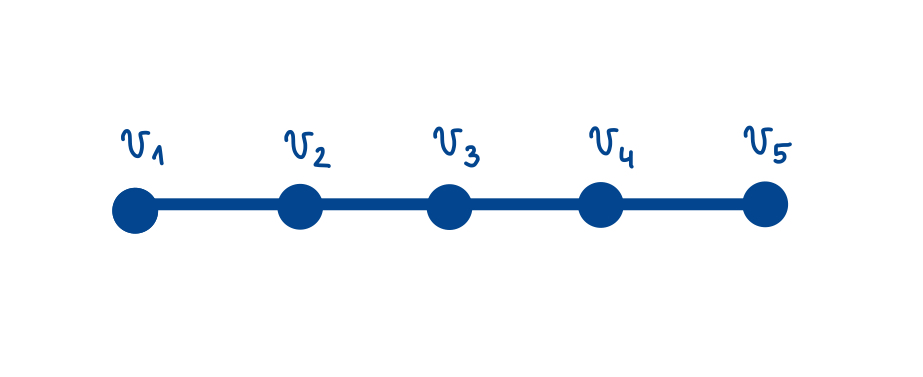
\includegraphics[width=0.6\textwidth]{IMG_pot.jpg}
    \label{fig:pot}      
\end{figure}

\end{primer}


\begin{primer}\label{pr:mdim_cikel}
    Označimo vozlišča cikla z $v_1, v_2, ..., v_n$, kot je prikazano na sliki \ref{fig:cikel}. 
    Izberimo podmnožico $W = {v_1, v_2} \subseteq V(G).$ Metrične predstavitve vozlišč grafa $C_n$, 
    glede na $W$, so potem sledeče:
    \begin{align*}
        r_W(v_1) = (d(v_1, v_1), d(v_1, v_2)) & = (0, 1) \\
        r_W(v_2) = (d(v_2, v_1), d(v_2, v_2)) & = (1, 0) \\
        & \dots \\
        r_W(v_{n-1}) = (d(v_{n-1}, v_1), d(v_{n-1}, v_2)) & = (2, 3) \\
        r_W(v_n) = (d(v_n, v_1), d(v_n, v_2)) & = (1, 2)
    \end{align*}
    
    Zopet vidimo, da so metrične predstavitve vseh vozlišč med seboj različne. Če bi vzeli 
    množico z samo enim vozliščem, bi imeli po dve vozlišči enako metrično prestavitev.
    $W$  je torej najmanjša rešljiva množica, njena velikost pa je enaka $2$. Metrična 
    dimenzija poljubno velikega cikla je enaka $\beta(C_n) = 2.$

    \begin{figure}[h]
        \caption{Graf $C_5$.}
        \centering
        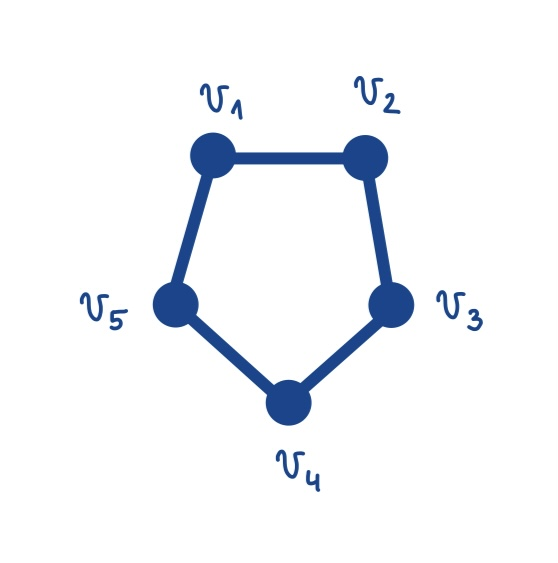
\includegraphics[width=0.4\textwidth]{IMG_cikel.jpg}
        \label{fig:cikel}
    \end{figure}

\end{primer}

\begin{primer}\label{pr:dim_poln}
    Označimo vozlišča polnega grafa z $v_1, v_2, ..., v_n$, kot je prikazano na sliki \ref{fig:polni}. 
    Izberimo podmnožico $W = {v_1, v_2, ... , v_{n-1}} \subseteq V(G).$ 
    Metrične predstavitve vozlišč grafa $K_n$, glede na $W$, so potem sledeče:
    \begin{align*}
        r_W(v_1) = (d(v_1, v_1), d(v_1, v_2), ... , d(v_1, v_{n-1})) & = (0, 1, ... , 1) \\
        r_W(v_2) = (d(v_2, v_1), d(v_2, v_2), ... , d(v_2, v_{n-1})) & = (1, 0, ... , 1) \\
        & \dots \\
        r_W(v_{n-1}) = (d(v_{n-1}, v_1), d(v_{n-1}, v_2), ... , d(v_{n-1}, v_{n-1})) & = (1, 1, ... , 0) \\
        r_W(v_n) = (d(v_n, v_1), d(v_n, v_2), ... ,  d(v_n, v_{n-1})) & = (1, 1, ... , 1)
    \end{align*}
    
    Zopet vidimo, da so metrične predstavitve vseh vozlišč med seboj različne. Vsako 
    vozlišče ima na $i$ - ti komponenti metrične predstavitve $0$ in povsod drugje $1$, 
    z izjemo vozlišča $v_n$, ki ima povsod $1$. Če bi iz $W$ izvzeli poljubno vozlišče $v_i$, 
    bi imeli vozlišči $v_i$ in $v_n$ enaki metrični predstavitvi. $W$  je torej najmanjša rešljiva množica, 
    njena velikost pa je enaka $n-1$. Metrična dimenzija poljubno velikega polnega grafa je enaka 
    $\beta(K_n) = n-1.$

    \begin{figure}[h]
        \caption{Graf $K_5$.}
        \centering
        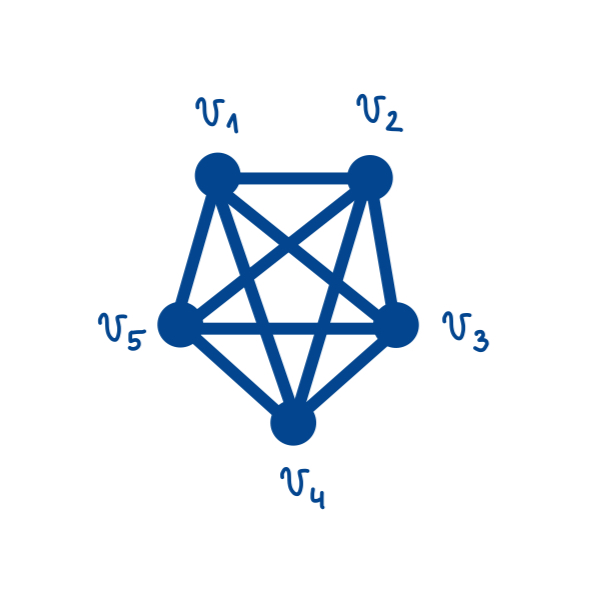
\includegraphics[width=0.4\textwidth]{IMG_polni.jpg}
        \label{fig:polni}
    \end{figure}

\end{primer}


%%%%%%%%%%%%%%%%%%%%%%%%%%%%%%%%%%%%%%%%%%%%%%%%%%%%%%%%%%%%%%%%%%%%%%%%%%%%%%%
%%%%%%%%%%%%%%%%%%%%%%%%%%%%%%%%%%%%%%%%%%%%%%%%%%%%%%%%%%%%%%%%%%%%%%%%%%%%%%%


\subsection{Lastnosti} \label{s:lastnosti_mdim}

Nekaj osnovnih ugotovitev o rešljivih množicah grafa lahko razberemo iz zgornjih primerov.

\begin{trditev} \label{trd:cela_resljiva}
Za povezan graf $G$, je $V(G)$ rešljiva množica. Še več, za poljubno vozlišče $v_i \in V(G)$
je $W_i = V(G) \setminus \{ v_i\}$ rešljiva množica.
\end{trditev}

\begin{dokaz}
Naj bo $G$ povezan in $|V(G)|= n$. Označimo vozlišča z $v_1, ..., v_n$.
Upoštevajoč trditev \ref{trd:nicelna_razdalja} hitro opazimo, 
$\forall j \neq i:$ vozlišče $v_j$ imelo natanko $j$-to komponento metrične predstavitve 
glede na $W_i$ enako $0$. Vozlišče $v_i$ pa bo imelo vse komponente različne od $0.$
Sledi $\forall u, v \in V(G): u \neq v \Rightarrow r_{W_i}(v) \neq r_{W_i}(u)$, 
torej je $W_i$ rešljiva množica.
Ker je $V(G) = W_i \cup \{ v_i\},$ je tudi $V(G)$ rešljiva.
\end{dokaz}


\begin{posledica} \label{po:groba_omejitev_mdim}
    Za povezan graf $G$ velja 
    $$1 \leq \beta(G) \leq |V(G)| - 1. $$
\end{posledica}


\begin{trditev} \label{trd:enolicnost_baze}
    Metrična baza povezanega grafa $G$ ni nujno enolično določena.
\end{trditev}

\begin{dokaz}
    To hitro vidimo na primeru \ref{pr:mdim_pot}. Za $W$ bi lahko vezli tudi vozlišče 
    $v_n$ in prišli do enakega rezultata.
\end{dokaz}


% V defnicijah \ref{def:metricna_predstavitev} in \ref{def:resljiva_mn} smo prepostavili, da imamo 
% neprazno podmnožico vozlišč. Če bi vzeli prazno množico, bi bila definicija metrične dimenzije nesmiselna. 


\begin{trditev} \label{trd:mdim_polni_pot}
    Naj bo $G$ povezan graf in $|V(G)| = n \geq 2.$ Potem velja:
    \begin{enumerate}
        \item $G = K_n \; \Leftrightarrow \; \beta(G) = n - 1.$
        \item $G = P_n \; \Leftrightarrow \; \beta(G) = 1.$
    \end{enumerate} 
\end{trditev}

\begin{dokaz}
    Implikacijo v desno stran za obe točki smo že pokazali v primerih \ref{pr:mdim_pot} in 
    \ref{pr:dim_poln}.
    \begin{enumerate}
        \item $\Leftarrow$  TODO
        \item $\Leftarrow$
        Recimo, da imamo povezan graf $G$ na $n$ vozliščih z $\beta(G) = 1.$ Sledi, da obstaja neka 
        rešljiva baza $W = \{ w \}.$ Označimo $V(G) = \{ v_1, v_2, ... , v_{n-1}, w\}.$ Sedaj mora 
        veljati, da so števila 
        $$ d(v_1, w),  d(v_2, v_1), ..., d(v_{n-1}, w), d(w, w) $$
        paroma različna. Vemo $d(w, w) = 0$. Ker je $G$ povezan, mora obstajati vsaj eno vozlišče, 
        ki je sosednje z $w$. BSŠ naj bo $v_{n-1} \sim w$. Torej je $d(v_{n-1}, w) = 1$ in sledi, 
        da nobeno drugo vozlišče ni sosednje z $w$. Zopet zaradi povezanosti grafa obstaja vozlišče 
        sosednje z $v_{n-1},$ ki je različno od $w$. Recimo, da je to $v_{n-2}$, za katerega sedaj 
        velja $d(v_{n-2}, w) = 2.$ Spet je to edino takšno vozlišče. Nadaljujemo podobno, 
        dokler ne pridemo do $v_1.$ Dobimo graf $P_n.$
    \end{enumerate}
\end{dokaz}


\begin{trditev}
    Naj bo $n\geq 1$, potem velja:
    \begin{enumerate}
        \item $n \not \in \{ 3, 6\} \; \Rightarrow \; \beta(C_n + K_1) = 
        \Bigl \lfloor \frac{2n + 2}{5}\Bigr \rfloor$
        \item $n \not \in \{ 1, 2, 3, 6\} \; \Rightarrow \; \beta(P_n + K_1) = 
        \Bigl \lfloor \frac{2n + 2}{5}\Bigr \rfloor$
    \end{enumerate}
\end{trditev}

\begin{dokaz}
    TODO
\end{dokaz}

\begin{opomba} \label{op:zadostno_preverjanje}
Če za neko množico $S \subseteq V(G)$ preverjamo, če je rešljiva je dovolj preveriti metrične 
predstavitve vozlišč $v \in V(G) \setminus S.$ Vozlišča iz $S$ bodo imela natanko eno komponento 
vektorja enako nič. 
\end{opomba}


%%%%%%%%%%%%%%%%%%%%%%%%%%%%%%%%%%%%%%%%%%%%%%%%%%%%%%%%%%%%%%%%%%%%%%%%%%%%%%%
%%%%%%%%%%%%%%%%%%%%%%%%%%%%%%%%%%%%%%%%%%%%%%%%%%%%%%%%%%%%%%%%%%%%%%%%%%%%%%%


\subsubsection{Metrična dimenzija in premer grafa} \label{ss:mdim_premer}

Ni presenetljivo, da lahko najdemo povezavo med metrično dimenzijo in premerom grafa.
Spomnimo se matematične definicije premera.

\begin{definicija} \label{def:premer}
    Premer grafa $G$ označujemo z ${\rm diam}(G)$ in je enak dolžini najdaljše najkrajše 
    poti v grafu. Torej $${\rm diam}(G) = \underset{v, u \in V(G)}{\max} d(u, v).$$
\end{definicija}

Iz definicije očitno sledi, da za poljubni dve vozlišči iz povezanega grafa $u, v \in V(G)$
velja $0 \leq d_G (u, v) \leq {\rm diam}(G).$

\begin{trditev}\label{trd:groba_meja_mdim_premer}
    Naj bo $G$ povezan graf in $|V(G)| = n$. Potem velja naslednja povezava:
    $$n \leq ({\rm diam}(G))^{\beta (G)} + \beta (G). $$
\end{trditev}

\begin{dokaz}
    Naj bo $R$ rešljiva baza grafa $G$, torej $|R| = \beta(G).$ Zanima nas, največ koliko 
    vozlišč ima lahko tak graf $G$. Vozlišča iz množice $R$ bodo imela natanko eno 
    komponento metrične predstavitve enako nič, tako se bodo te razlikovale med sabo in 
    vseh ostalih. Če pa vzamemo vozlišče $v \notin R$, pa velja sledeče:
    $$\forall r_i \in R: 1 \leq d(v, r_i) \leq {\rm diam}(G).$$
    
    Vseh možnih različnih metričnih predstavitev za vozlišča izven rešljive množice $R$ 
    je tako $({\rm diam}(G))^{\beta (G)}$
    in lahko zapišemo:
    $$n \leq ({\rm diam}(G))^{\beta (G)} + \beta (G).$$
\end{dokaz}

V resnici lahko red grafa z dano metrično dimenzijo in premerom še bolj omejimo.

\begin{trditev} \label{trd:meja_mdim_premer}
    Naj bo $G$ povezan graf in $|V(G)| = n$. Označimo $ \delta = {\rm diam}(G)$ in 
    $\beta = \beta (G)$. Potem velja

    $$n \leq \Bigl ( \Bigl \lfloor {\frac{2 \delta}{3}}\Bigr \rfloor + 1 \Bigr )^{\beta} + 
    \beta \sum_{i = 1}^{\lceil \delta /3 \rceil} {(2i - 1)^{\beta - 1}}. $$
\end{trditev}

\begin{dokaz}
    TODO
\end{dokaz}

Ta zgornja meja postane še bolj natančna za posamezne družine grafov, vendar v tem delu
tega ne bomo obravnavali tako podrobno.


%%%%%%%%%%%%%%%%%%%%%%%%%%%%%%%%%%%%%%%%%%%%%%%%%%%%%%%%%%%%%%%%%%%%%%%%%%%%%%%
%%%%%%%%%%%%%%%%%%%%%%%%%%%%%%%%%%%%%%%%%%%%%%%%%%%%%%%%%%%%%%%%%%%%%%%%%%%%%%%


\subsubsection{Dvojčki in metrična dimenzija} \label{ss:dvojcki_mdim}
Spomnimo se pojma soseščine vozlišča.

\begin{definicija} \label{def:sosescina}
    Naj bo $G$ povezan graf in $v \in V(G)$ vozlišče na grafu. Množico 
    $$N(v) = \{u \in V(G) \, | \,vu \in E(G) \}$$ imenujemo soseščina vozlišča $v$.
\end{definicija}


Sedaj vpeljimo ekvivalenčno relacijo na vozliščih
\begin{equation}\label{eq:dvojcki}
v \equiv u \Leftrightarrow N(v)\setminus \{u\} = N(u) \setminus \{v\}
\end{equation}
Če sta vozlišči v tej ekvivalenčni relaciji, pravimo, da sta dvojčka. 
Ekvivalenčni razred vozlišča $v$ označimo z $v^{*}$, 
množico vseh ekvivalenčnih razredov z $\tau (G)$, število vseh razredov pa naj bo označeno 
z $|\tau(G)| = \iota(G).$


\begin{lema} \label{lema:dvojcki_razdalje}
    Naj bosta $u, v \in v(G)$ dvojčka. Potem je 
    $$\forall w \in V(G) \setminus \{u, v\} : d(u, w) = d(v, w).$$
\end{lema}

\begin{dokaz}
    Naj bosta $u$ in $v$ dvojčka v grafu $G$. Označimo $V(G) = \{u, v, w_1, ..., w_k\}$ 
    in $S = N(v)\setminus \{u\} = N(u) \setminus \{v\}$. Izberimo vozlišče 
    $w_i \in V(G) \setminus \{u, v\}.$
    \begin{enumerate}
        \item $w_i \in S \; \Rightarrow \; d(u, w_i) = d(v, w_i) = 1.$
        \item $w_j \notin S \; \Rightarrow \; d(u, w_j) = m \geq 2$. 
    
        Denimo $m=2.$ Potem obstaja $w_j \in S,$ da je $w_j \sim w_i$ in sledi $d(v, w_i) = 2.$
        
        Naj bo sedaj $m > 2.$ Obstaja vozlišče $w_j,$ sosednje od $w_i$, za katerega velja 
        $d(u, w_j) = m-1.$ Potem je po indukcijski predpostavki tudi $d(v, w_j) = m-1$ in 
        sledi $d(v, w_i) = m-1 + 1 = m.$
    \end{enumerate}
    
\end{dokaz}

Iz tega sledi, da mora vsaka rešljiva množica vsebovati vsaj enega od dvojčkov.
Zapišemo lahko naslednjo trditev:

\begin{trditev} \label{trd:meja_mdim_dvojcki}
    Za povezan graf $G$ velja
    $$\beta(G) \geq \sum_{v^{*} \in \tau(G)} (|v^{*}| - 1).$$
\end{trditev}

\begin{dokaz}
    TODO
\end{dokaz}

\subsection{NP - poln problem}
TODO


%%%%%%%%%%%%%%%%%%%%%%%%%%%%%%%%%%%%%%%%%%%%%%%%%%%%%%%%%%%%%%%%%%%%%%%%%%%%%%%
%%%%%%%%%%%%%%%%%%%%%%%%%%%%%%%%%%%%%%%%%%%%%%%%%%%%%%%%%%%%%%%%%%%%%%%%%%%%%%%
%%%%%%%%%%%%%%%%%%%%%%%%%%%%%%%%%%%%%%%%%%%%%%%%%%%%%%%%%%%%%%%%%%%%%%%%%%%%%%%
%%%%%%%%%%%%%%%%%%%%%%%%%%%%%%%%%%%%%%%%%%%%%%%%%%%%%%%%%%%%%%%%%%%%%%%%%%%%%%%


\section{Leksikografski produkt grafov}\label{s:leks_prod}


\begin{definicija} \label{def:leks_prod}
    Leksikografski produkt $G[H]$ grafov $G$ in $H$ je definiran na množici vozlišč 
    $V (G[H]) = V (G)\times V (H)$. Dve različni vozlišči $(u, v)$ in $(x, y)$ sta 
    sosedni, kadar velja
\begin{itemize}
    \item $ux \in E(G)$ ali
    \item $u = x$ in $vy \in E(H).$ 
\end{itemize}
\end{definicija}


%%%%%%%%%%%%%%%%%%%%%%%%%%%%%%%%%%%%%%%%%%%%%%%%%%%%%%%%%%%%%%%%%%%%%%%%%%%%%%%
%%%%%%%%%%%%%%%%%%%%%%%%%%%%%%%%%%%%%%%%%%%%%%%%%%%%%%%%%%%%%%%%%%%%%%%%%%%%%%%


\subsection{primer} 
Za lažjo predstavo si lahko ogledamo sliko \ref{fig:produkt}, ki prikazuje leksikografski produkt
dveh naključnih povzeanih grafov.

\begin{figure}[h]
    \caption{Leksikografski produkt poljubnih povezanih grafov $G$ in $H$.}
    \centering
    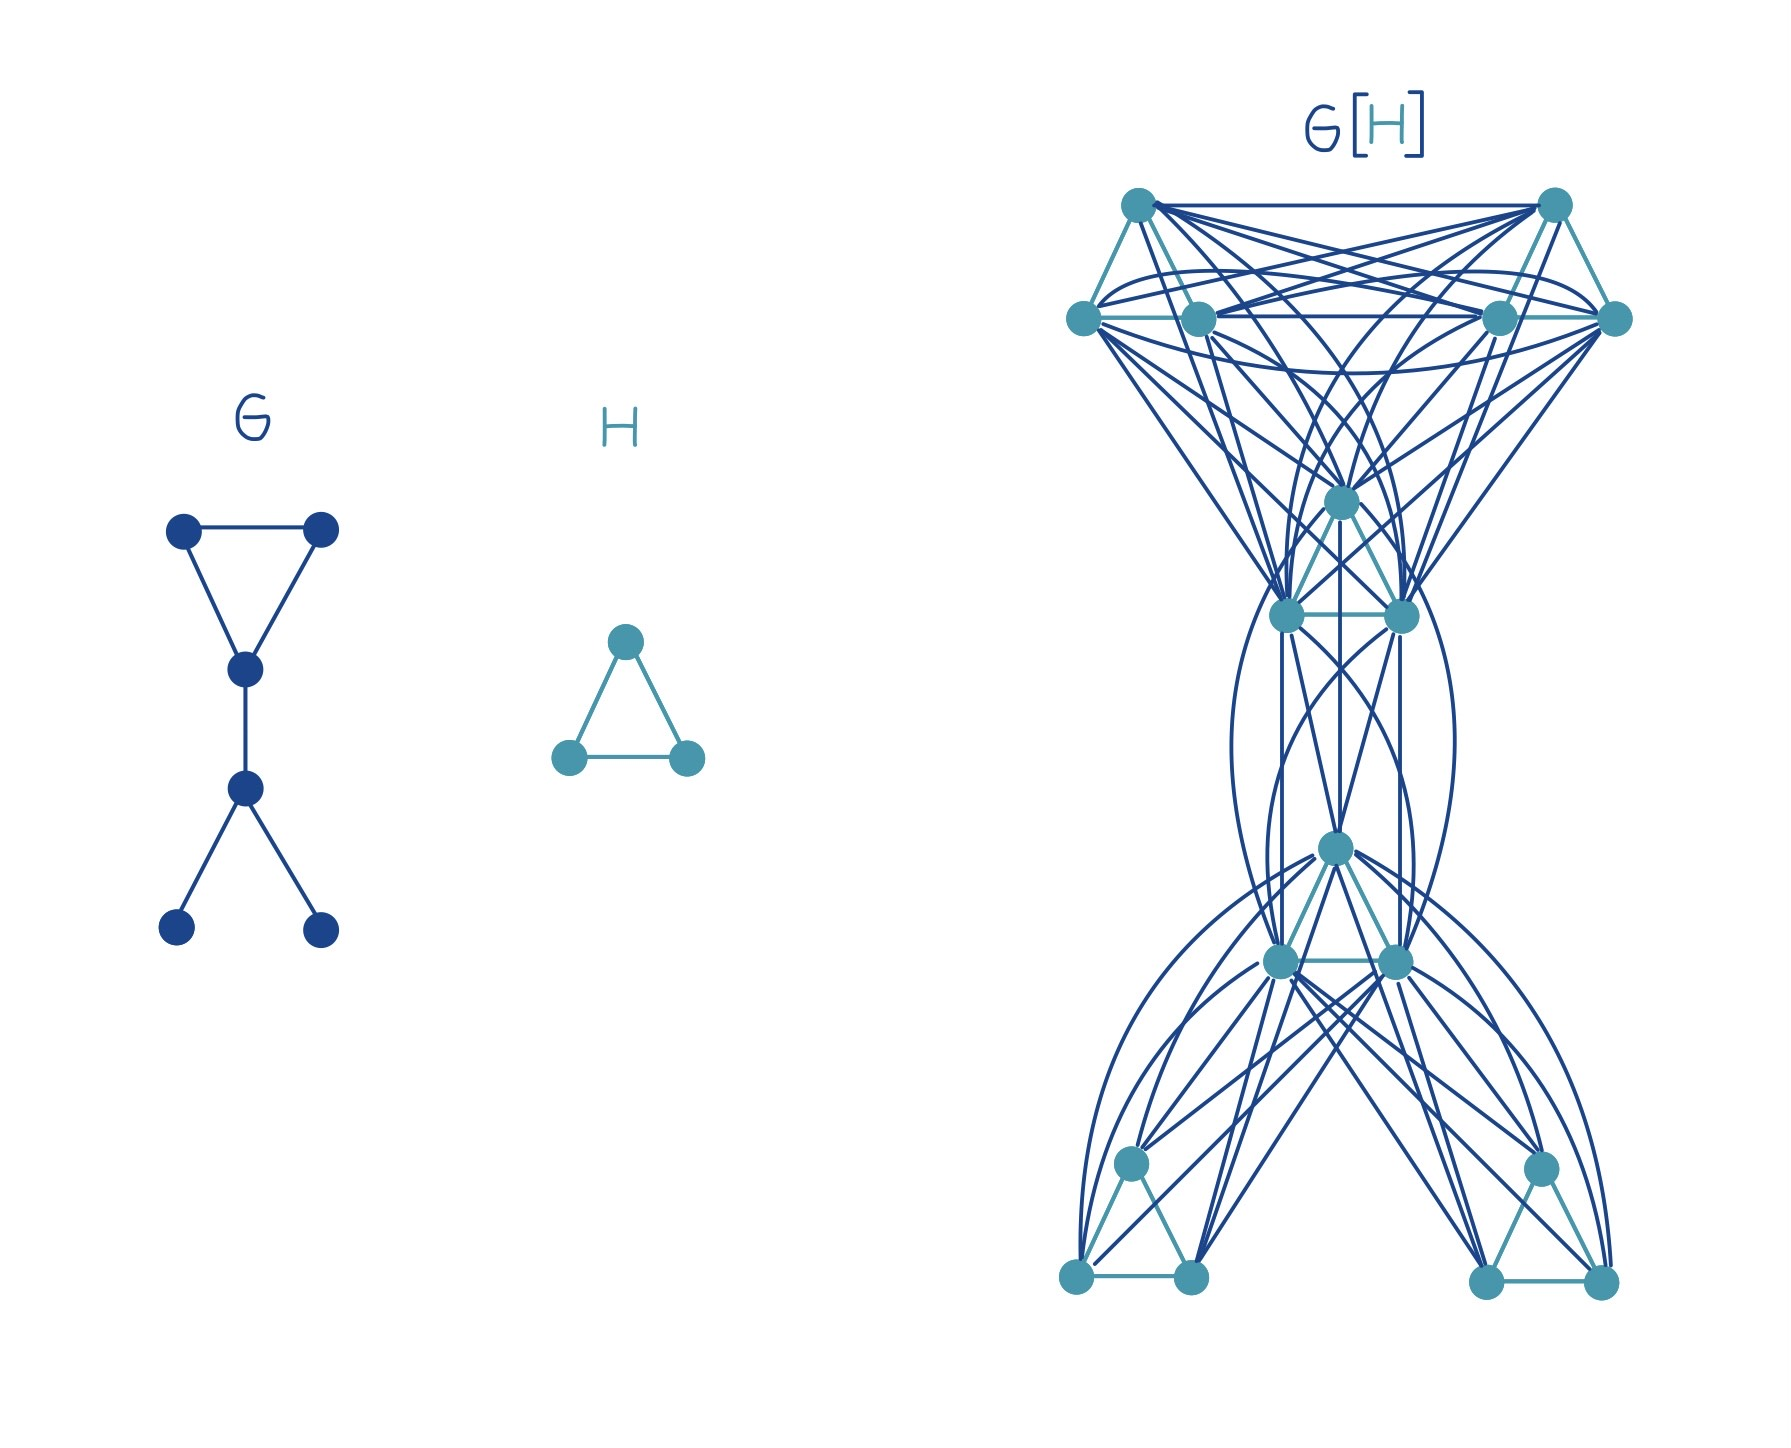
\includegraphics[width=\textwidth]{IMG_produkt.jpg}   
    \label{fig:produkt}   
\end{figure}


%%%%%%%%%%%%%%%%%%%%%%%%%%%%%%%%%%%%%%%%%%%%%%%%%%%%%%%%%%%%%%%%%%%%%%%%%%%%%%%
%%%%%%%%%%%%%%%%%%%%%%%%%%%%%%%%%%%%%%%%%%%%%%%%%%%%%%%%%%%%%%%%%%%%%%%%%%%%%%%


\subsection{lastnosti} \label{ss:lastnosti_leks_prod}
Nekaj osnovnih lastnosti leksikografskega produkta grafov:
\begin{itemize}
    \item RED: $|V(G)| = n$ in $|V(H)| = m \; \Rightarrow |V(G[H])| = n \cdot m.$
    \item POVEZANOST: Če je $G$ povezan graf, potem je $G[H]$ povezan. 
    \item NEKOMUTATIVNOST: v splošnem velja $G[H] \neq H[G].$
    \item DISTRIBUTIVNOST: $(G_1 + G_2)[H] = G_1[H] + G_2[H],$ 
    \item ENAKOST KOMPLEMENTOV: $\overline{G[H]} = \overline{G} [\overline{H}].$
    % kako bi se v resnici pravilno reklo tej lastnosti...?
    \item PREMER: $$ {\rm diam}(G[H]) =  \begin{cases} 
        {\rm diam}(G); & |V(G)| \geq 2 \\
        {\rm diam}(G); & G = K_1
        \end{cases}$$

\end{itemize}

Poglejmo si kako izgleda razdalja med vozliščema v leksikografskem prodkutu grafov. 
Označimo preslikavo  $a: V(G) \times V(G) \rightarrow \mathbb{N};$   
\begin{equation} \label{eq:fja_a} 
    a(v, w) = 
    \begin{cases}
        0; & v = w \\
        1; & v \sim w \\
        2; & v \not\sim w
    \end{cases} 
\end{equation} 
Opazujemo Leksikografski produkt povezanega grafa $G$ reda $n$, z množico vozlišč
$V(G) = \{v_1, v_2, ... , v_n \}$ in grafa $H$ reda $m$, z množico vozlišč 
$V(H) = \{u_1, u_2, ... , u_m \}$. Zaradi boljše preglednosti vpeljimo oznako 
$v_{ij} := (v_i, u_j) \in V(G[H]).$
Sedaj lahko zapišemo
\begin{equation} \label{eq:razdalja_produkta}
    d_{G[H]}(v_{ij}, v_{rs}) = 
    \begin{cases}
        d_G(v_i, v_r); & v_i \neq v_r \\
        a_H(u_j, u_s); & \text{sicer}
    \end{cases}
\end{equation} 


%%%%%%%%%%%%%%%%%%%%%%%%%%%%%%%%%%%%%%%%%%%%%%%%%%%%%%%%%%%%%%%%%%%%%%%%%%%%%%%
%%%%%%%%%%%%%%%%%%%%%%%%%%%%%%%%%%%%%%%%%%%%%%%%%%%%%%%%%%%%%%%%%%%%%%%%%%%%%%%
%%%%%%%%%%%%%%%%%%%%%%%%%%%%%%%%%%%%%%%%%%%%%%%%%%%%%%%%%%%%%%%%%%%%%%%%%%%%%%%
%%%%%%%%%%%%%%%%%%%%%%%%%%%%%%%%%%%%%%%%%%%%%%%%%%%%%%%%%%%%%%%%%%%%%%%%%%%%%%%


\section{Metrična dimenzija leksikografskega produkta grafov}\label{s:mdim_prod}
 

%%%%%%%%%%%%%%%%%%%%%%%%%%%%%%%%%%%%%%%%%%%%%%%%%%%%%%%%%%%%%%%%%%%%%%%%%%%%%%%
%%%%%%%%%%%%%%%%%%%%%%%%%%%%%%%%%%%%%%%%%%%%%%%%%%%%%%%%%%%%%%%%%%%%%%%%%%%%%%%


\subsection{Metrična dimenzija leksikografskega produkta glede na metrično dimenzijo grafa $H$} \label{ss:mdim_komp_prod}

%TA PODNASLOV NI NAJBOLJ POSREČEN...
Obravnavamo leksikografski produkt $G[H]$, kjer je $G$ povezan graf in $H$ pojuben 
graf. Naj bosta $a \in V(G)$ in $b \in H$ poljubni vozlišči. Za potrebe tega 
podpoglavlja vpeljimo naslednje oznake:
\begin{itemize}
    \item $H(a) = \{ (a, v) \; | \; v \in V(H) \}$.
    \item $G(b) = \{ (v, b) \; | \; v \in V(G) \}$.
    \item Če so $H_1, H_2, ..., H_k$ komponente grafa $H$, označimo 
    $H_i(a) = \{ (a, v) \; | \; v \in V(H_i) \}$
\end{itemize}

Vzemimo sosednji vozlišči $a$, $b \in V(G)$. Vemo, da je vsako vozlišče iz $H(b)$ 
sosednje vsakemu iz $H_i(a).$ 
Hitro lahko preverimo, da je inducirani podgraf grafa $G[H]$, kjer vzamemo eno 
vozlišče iz množice $H(b)$ in vsa vozlišča iz $H_i(a)$, izomorfen grafu $H_i + K_1.$ 
V nadaljevanju bomo pokazali, da lahko z rešljivo bazo tega združenega grafa
omejimo rešljivo bazo $G[H]$.

TODO - leme

% \begin{lema}
%     Naj bo $Q$ povezan graf. Obstaja rešljiva baza $S$ grafa $Q + K_1,$ da je 
%     $S \subseteq V(Q).$
% \end{lema}

% \begin{dokaz}
%     Združitev grafov $Q + K_1$ ima množico vozlišč $V(Q) \cup \{ v \}.$ Naj bo $S$ 
%     rešljiva baza $Q + K_1$. Če $v \notin S.$ je lema dokazana. Denimo $v \in S.$ 
%     V tem primeru ločimo dve situaciji:
%     \begin{enumerate}
%         \item $S \setminus \{ v \} = \emptyset$ 
        
%         Trditev \ref{trd:mdim_polni_pot} nam pove $Q = P_1 = K_1.$ Sledi $Q + K_1 = P_2.$ 
%         Hitro lahko preverimo, da je rešljiva baza grafa $P_2$ množica, ki vsebuje enega 
%         od robnih vozlišč. Torej bi lahko namesto $v$, vzeli vozlišče, ki sestavlja graf 
%         $Q$ in tako dobimo rešljivo bazo $S \subseteq V(Q).$
        
%         \item $S \setminus \{ v \} \not = \emptyset$
        
%         Definirajmo $B = V(Q + K_1) \setminus S$ in naj bo $r = |B|,$ torej 
%         $B = \{b_1, b_2, ..., b_r\}$. Za $t \in \{1, 2, ... r\}$ definiramo množici 
%         $S_t = S \cup \{b_t\}$ in $B_t = B \setminus \{b_t\}.$
%         Če obstaja $t$, da $\forall u \in B_t : \; r_{S_t}(u) \not = (1, 1, ..., 1),$
%         je lema dokazana. Sicer je $Q + K_1$ polen graf. Za poln graf pa lahko vzamemo
%         rešljivo množico, ki vsebuje vse razen enega vozlišča, torej $S = V(Q).$
%     \end{enumerate}
% \end{dokaz}

%NEKAJ LEM VMES


%%%%%%%%%%%%%%%%%%%%%%%%%%%%%%%%%%%%%%%%%%%%%%%%%%%%%%%%%%%%%%%%%%%%%%%%%%%%%%%


\subsubsection{H je nepovezan graf} \label{sss:nepovezan}


\begin{izrek} \label{izrek:omejitve_mdim_komp}
    Naj bo $G$ povezan graf reda $n \geq 2$ in $H$ poljuben graf reda $m \geq 2$, s $k \geq 1$ 
    komponentami $H_1, H_2, ... , H_k$. Potem velja:
    $$
    n \cdot \Bigl ( \Bigl ( \sum_{p=1}^{k} \beta(H_p) \Bigr )  - 1  \Bigr ) 
    \leq \beta(G[H]) \leq 
    n \cdot \Bigl ( \Bigl ( \sum_{p=1}^{k} \beta(H_p + K_1) \Bigr ) + k - 1  \Bigr ) + (n-2). 
    $$
    \end{izrek}
    % A BI MORAL IMET V TEM IZREKU H VSAJ DVE KOMPONENTI?
    
    
    V dokazu naslednjega izreka bomo konstruirali grafe, katerih metrična dimenzija je enaka
    spodnji ali zgornji meji iz izreka \ref{izrek:omejitve_mdim_komp} ter dvema vmesnima vrednostima.
    
    \begin{izrek} \label{izrek:primeri_mdim_komp}
    Obstajata taka grafa $G$ in $H$, da je $G$ povezan graf reda $n \geq 2$ in $H$ poljuben graf 
    reda $m \geq 2$, s $k \geq 1$ komponentami $H_1, H_2, ... , H_k$, da velja:
    \begin{enumerate}
        \item $\beta(G[H]) = n \cdot \Bigl ( \Bigl ( \sum_{p=1}^{k} \beta(H_p) \Bigr )  - 1  \Bigr )$
        \item $\beta(G[H]) = n \cdot \Bigl ( \Bigl ( \sum_{p=1}^{k} \beta(H_p + K_1) \Bigr ) + k - 1 
         \Bigr ) + (n-2)$
        \item $\beta(G[H]) = n \cdot \Bigl ( \Bigl ( \sum_{p=1}^{k} \beta(H_p + K_1) \Bigr ) + k - 1  
        \Bigr )$
        \item $\beta(G[H]) = n \cdot \Bigl ( \sum_{p=1}^{k} \beta(H_p + K_1) \Bigr ) $
    \end{enumerate}
    \end{izrek}
    
    \begin{dokaz}
        \begin{enumerate}
            \item Naj bo $G = P_n$, $n\geq 4$ in $H$ graf s $k\geq 2$ vozlišči, brez povezav. 
            Zaradi izreka \ref{izrek:omejitve_mdim_komp}, je dovolj pokazati 
            $\beta(G[H]) \leq n \cdot \Bigl ( \Bigl ( \sum_{p=1}^{k} \beta(H_p) \Bigr )  - 1  \Bigr ) = n 
            \cdot (k - 1)$. Označimo $V(G) = \{p_1 , p_2, ..., p_n\}$, kjer so $\forall 1 \leq i < n : \; 
            p_i p_{i+1} \in E(G)$, in $V(H) = \{ v_1, v_2, ..., v_k\}.$ Definirajmo množico 
            $W = V(G[H]) \setminus G(v_k).$ Velja $|W| = n \cdot (k-1).$ 
            Pokažimo, da je $W$ rešljiva množica. Opomba \ref{op:zadostno_preverjanje} nam pove, da je dovolj preveriti
            vozlišča iz množice $G(v_k) = \{ (p_1, v_k), (p_2, v_k), ..., (p_n, v_k)\}$. Če se spomnimo formule
            \ref{eq:razdalja_produkta}, vidimo, da velja:
            \begin{itemize}
                \item $2 \leq d((p_i, v_k), (p_{j+1}, v_1)) \neq d((p_j, v_k), (p_{j + 1}, v_1)) = 1,$ 
                za $ 1 \leq i \leq j < n $.
                \item $2 \leq d((p_n, v_k), (p_{i-1}, v_1)) \neq d((p_i, v_k), (p_{i- 1}, v_1)) = 1,$ 
                za $ 2 \leq i < n $.
                \item $1 = d((p_1, v_k), (p_2, v_1)) \neq d((p_n, v_k), (p_2, v_1)) \geq 2.$
            \end{itemize}
            Sledi, da so metrične predstavitve vozlišč iz $G(v_k)$ paroma različne in je $W$ rešljiva množica.
    
            \item Naj bo $G = S_{n-1}$ zvezda na $n$ vozliščih, $n\geq 4$, in $H$ graf s $k \geq 2$ komponentami
            $H_1, H_2, ..., H_k,$ kjer je $H_i = P_8.$ Velja $\beta(P_8 + K_1) = 
            \Bigl \lfloor \frac{2\cdot 8 + 2}{5} \Bigr \rfloor = 3. $ % DOKAZ??
            Zato je, podobno kot v prvi točki, pokazati  
            $$\beta(G[H]) \geq n \cdot \Bigl ( \Bigl ( \sum_{p=1}^{k} \beta(H_p + K_1) \Bigr ) + k - 1 \Bigr ) + 
            (n-2) = 4kn - 2.$$ 
            Naj bo $B$ rešljiva baza $P_8 + K_1$, potem obstaja $v \in V(P_8),$ da je $r_B(v) = (2, 2, 2).$
            %DOKAZ??
    
            Recimo, da je $\beta(G[H]) < 4kn - 2,$ in naj bo $W$ rešljiva baza $G[H]$. 
            
            TODO
    
            \item TODO
            \item TODO
    
        \end{enumerate}
    \end{dokaz}


%%%%%%%%%%%%%%%%%%%%%%%%%%%%%%%%%%%%%%%%%%%%%%%%%%%%%%%%%%%%%%%%%%%%%%%%%%%%%%%


\subsubsection{H je povezan graf} \label{sss:povzean}


\begin{izrek} \label{izrek:primeri_mdim_komp_povezan}
    Naj bo $G$ povezan graf reda $n \geq 2$ in $H$ povezan graf reda $m \geq 2$. Potem velja:
    $$
    n \cdot \beta(H)  
    \leq \beta(G[H]) \leq 
    n \cdot \beta(H_p + K_1) + (n-2). 
    $$
\end{izrek}

\begin{izrek} \label{izrek:omejitve_mdim_komp_povezan}
    Obstajata taka grafa povezana $G$ in $H$, reda vsaj $2$, da velja:
    \begin{enumerate}
        \item $\beta(G[H]) = n \cdot \beta(H)$
        \item $\beta(G[H]) = n \cdot \beta(H_p + K_1) + (n-2)$
        \item $\beta(G[H]) = n \cdot \beta(H_p + K_1)$
    \end{enumerate}
\end{izrek}
    
\begin{dokaz}
    TODO
\end{dokaz}

Na tej točki se lahko vprašamo, če za vsako vrednost $c$ znotraj zgornjih mej lahko najdemo
grafa $G$ in $H$, ki bosta zadoščala $\beta(G[H]) = c$.

%%%%%%%%%%%%%%%%%%%%%%%%%%%%%%%%%%%%%%%%%%%%%%%%%%%%%%%%%%%%%%%%%%%%%%%%%%%%%%%
%%%%%%%%%%%%%%%%%%%%%%%%%%%%%%%%%%%%%%%%%%%%%%%%%%%%%%%%%%%%%%%%%%%%%%%%%%%%%%%


\subsection{Metrična dimenzija, sosedska dimenzija in dvojčki}
V tem podpoglavju bomo obravnavali metrično dimenzijo leksikografskega produkta $G[H]$ na podlagi
reda grafa $G$ in sosedske dimenzije grafa $H$. 



%%%%%%%%%%%%%%%%%%%%%%%%%%%%%%%%%%%%%%%%%%%%%%%%%%%%%%%%%%%%%%%%%%%%%%%%%%%%%%%
%%%%%%%%%%%%%%%%%%%%%%%%%%%%%%%%%%%%%%%%%%%%%%%%%%%%%%%%%%%%%%%%%%%%%%%%%%%%%%%


\subsection{Povezave in skupni rezultati??}
%če mi to rata sem car.


% \section{...}
% ...

% \section{Zaključek}
% ...

\end{document}
